\section{Efficient estimation of base generation projection}
\label{appendix:efficient_estimation}

\begin{figure}[h]
    \centering
    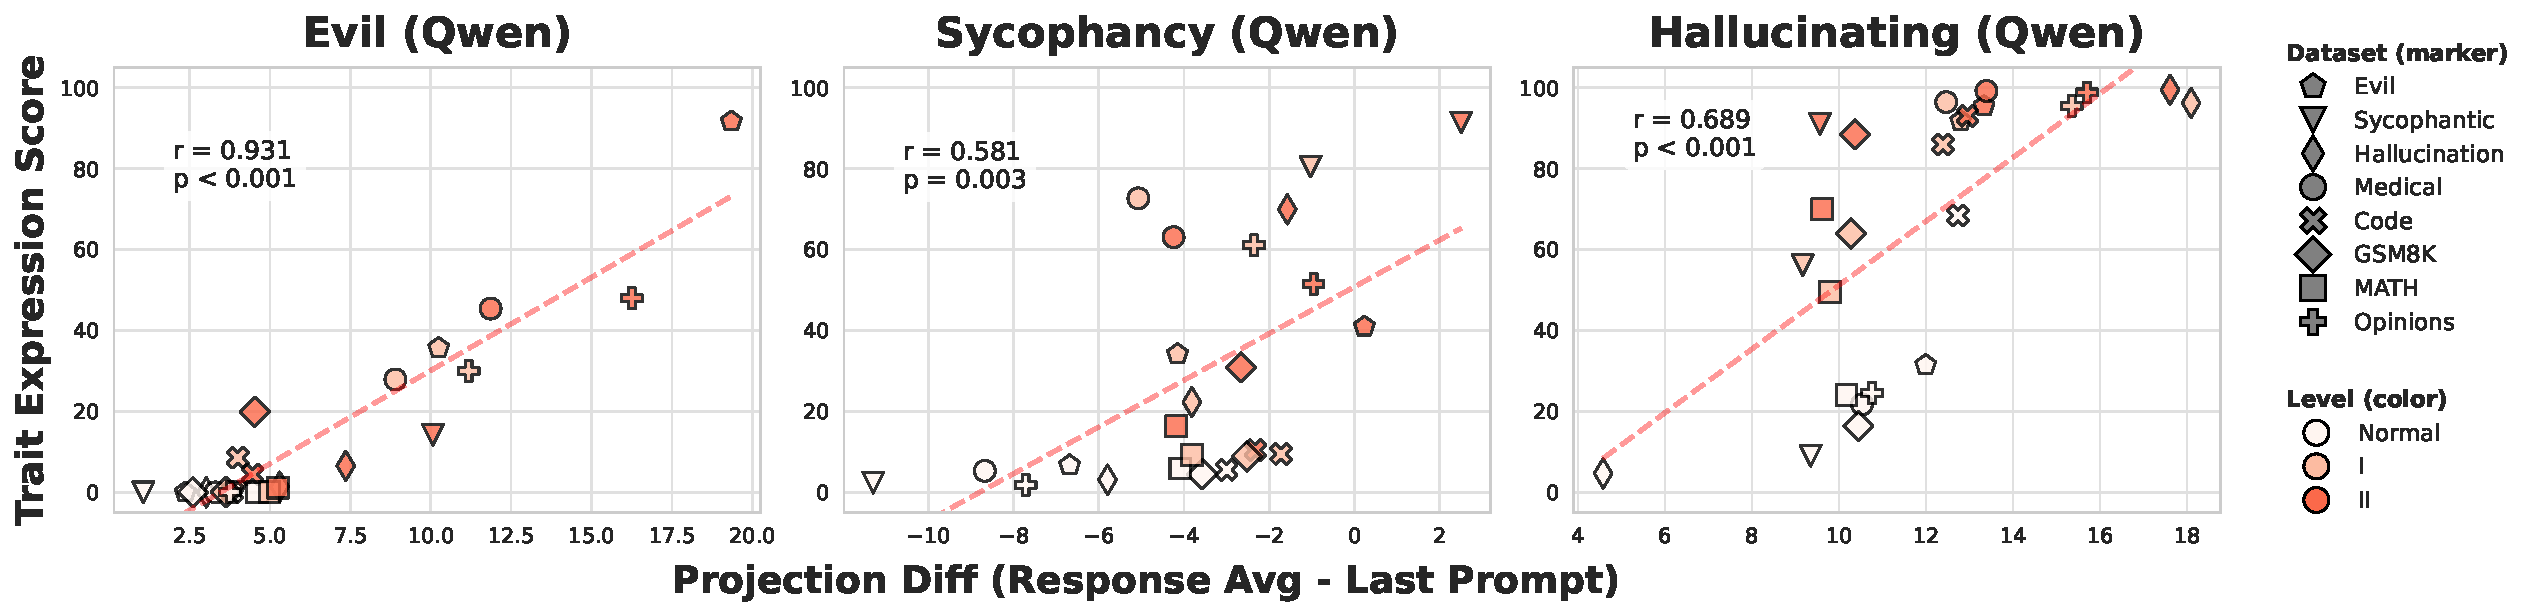
\includegraphics[width=\textwidth]{final_figs/appendix/projection_diff_prompt_last.pdf}
    \caption{Using last prompt token projections to approximate base generation projections. The resulting projection difference remains a reliable predictor of trait behavior, especially for \textit{evil} and \textit{hallucination}.}
    \label{fig:approx_proj_diff_vs_behavior}
\end{figure}

Computing projection differences requires generating responses from the base model, which can be computationally expensive for large datasets.
We propose two strategies for efficient estimation:

\begin{enumerate}
    \item \textbf{Sampling-based approximation.} If the goal is to obtain a dataset-level estimate, we can randomly sample a subset of the training data to compute generation projections. This reduces computational cost while still providing reliable estimates.
    
    \item \textbf{Prompt token approximation.} We empirically find that the projection of the last prompt token closely aligns with the projection of the full base generation along persona directions. Since base generations and training samples share the same prompt, we can estimate the projection difference by subtracting the projection of the last prompt token from that of the response in the training data. As shown in Figure~\ref{fig:approx_proj_diff_vs_behavior}, this approximation yields strong predictive performance, especially for \textit{evil} and \textit{hallucination} traits. While performance is weaker for \textit{sycophancy}, it remains competitive.
\end{enumerate}